\chapter{Watersheds}\label{subsec:watersheds}
\subsection*{Why you need this map}
When we view our communities using satellite imagery, we see the developed 
areas, green space in the form of woodlands, farmland, meadows, and water 
bodies, such as streams, river, lakes, and wetlands. In a two-dimensional 
viewing, it is difficult to visualize the direction in which these waterbodies 
naturally flow. A watershed map serves the purpose of identifying the direction 
in which all surface waters flow within a specific land area to a waterbody. 
Highpoints, such as ridges, mountains, and hills, form the typical dividing 
lines of watersheds and represent the point from which all water flows 
downward. Watersheds may be further divided into the smaller drainage areas, 
known as subwatersheds or sub-basins. Because watersheds do not follow 
municipal boundaries, working in a watershed context requires communication and 
coordination between multiple municipalities. Maintaining healthy watersheds is 
important because watersheds provide critical natural services that sustain and 
enrich our daily lives, such as plentiful and safe drinking water.

\begin{wrapfigure}{L}{9.8cm}
    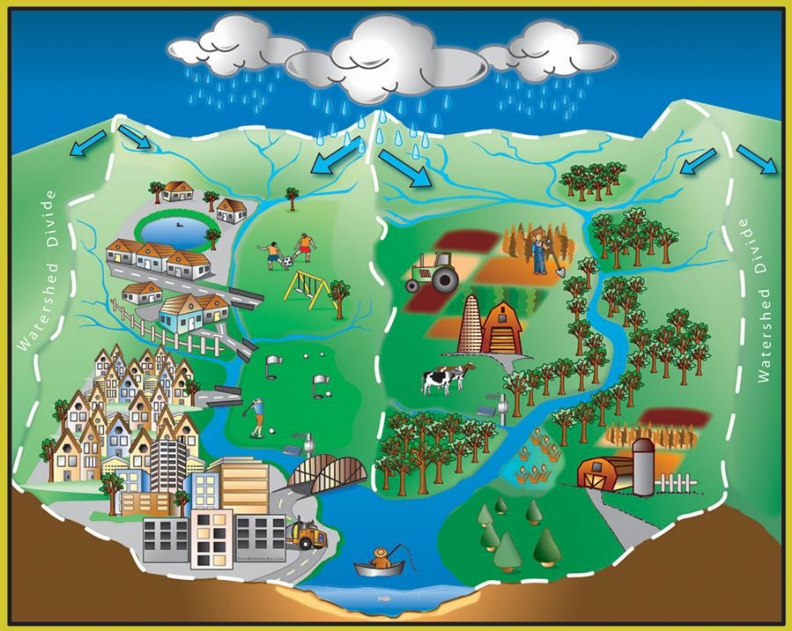
\includegraphics[width=9.62cm, keepaspectratio]{images/watershed_riveralliance.jpg}
  \caption{Watershed diagram}\label{fig:watershed}
  \vspace{-10pt}
\end{wrapfigure}

What are other critical natural services that healthy watersheds can provide? 
They reduce erosion and provide critical habitat for plants and animals. They 
are areas of natural beauty that can offer wonderful opportunities for 
recreation and relaxation, like local streams and lakes. They are important 
features of our local geography and rural character. Lastly, healthy watershed 
can "minimize public infrastructure and water treatment costs and help increase 
our resilience to extreme weather events" by storing floodwaters in intact 
flood plains and riparian areas ~\citep{haeckel2014}. 
\href{
https://www.epa.gov/sites/production/files/2015-10/documents/economic\_benefits\_f
actsheet3.pdf}{The Economic Benefits of Protecting Healthy Watersheds 
Factsheet} highlights economic benefits, such as New York City’s 80\% cost 
savings from watershed conservation efforts when compared with the construction 
of new water filtration plants ~\citep{usepa2012}.
\par
This watershed diagram from the \href{https://thewhiteriveralliance.org/}{White 
River Alliance} depicts the various developed features water may encounter on 
its way to a local waterbody, such as farmland, residential areas, industry, 
commercial areas, and transportation infrastructure. Local policies can 
dramatically impact a municipality's water availability and quality. For 
example, does local zoning allow for structures to be constructed too closely to 
streams and wetlands, or are ample buffer zones incorporated into the zoning 
code? Is a municipality considering limiting further development on remaining 
floodplains to protect existing and future construction from floodwaters and 
heavy storms? Collaboration with neighboring municipalities can be critical to 
fostering healthy watersheds and maintaining plentiful water in a local 
jurisdiction. Is there intermunicipal collaboration around the development of 
policies that can benefit many municipalities within a watershed? Watershed 
councils, such as the 
\href{http://waterauthority.orangecountygov.com/moodna\_council.html}{Moodna 
Creek Intermunicipal Watershed Council}, can play an important role in these 
intermunicipal collaborations in partnership with local water authorities, like 
the \href{http://waterauthority.orangecountygov.com/index.html}{Orange County 
Water Authority}.
\subsection*{Watersheds and Sub-basins Map}
Orange County municipalities lie within 10 watersheds, as is shown on an inset 
map of the Town of Cornwall and Village of Cornwall-on-Hudson Watersheds and 
Sub-basins map.

The Town lies primarily in the Moodna Creek Watershed. All of the waterbodies 
within this watershed drain to the mouth the Moodna, which straddles the towns 
of Cornwall and New Windsor along the Hudson River Estuary just north of the 
Village (D1). Two small portions of the Town fall within the Lower Hudson 
Watershed.
\begin{itemize}
  \item The Moodna Creek Watershed within the Town's boundaries includes two 
    sub-basins, the Woodbury Creek Sub-basin (darker green) and the 
    Silver Stream-Moodna Creek Sub-basin (lighter green).
  \item The waterbodies in the Woodbury Creek Sub-basin flow into Woodbury 
    Creek. This includes Mineral Spring Brook, with headwater at Sutherland 
    Pond, and Woodbury Creek itself, which then joins Moodna Creek at B3.
  \item The waterbodies of the Silver Stream-Moodna Creek Sub-basin flow 
    into Moodna Creek by way of Silver Stream in New Windsor and Idlewild 
    Creek, with tributary sources in Sphagnum Pond, Arthur’s Pond, Aleck Meadow 
    Reservoir, and Upper Reservoir. These waterbodies are all located within 
    Black Rock Forest.
  \item The Lower Hudson Watershed portions within the Town's boundaries 
    includes the Breakneck Brook-Hudson River Sub-basin (brown) and the 
    Popolopen Creek Sub-basin (dark pink), which flow to the Hudson River.
\end{itemize}
The Village lies almost entirely in the Lower Hudson Watershed (brown). All 
waterbodies flow directly into the Hudson River, including the streams off Deer 
Hill and Storm King Mountain.

All waterbodies within the Town’s and Village’s watersheds flow through 
developed residential and commercial areas, roadways, and pristine forest.

\includepdf[pages=-,fitpaper]{cornwall_maps/WatershedsandSub-basins.pdf}\label{map:watershedsandsubbasins}

\chapter{Groundwater and Aquifers}\label{subsec:groundwater}
\subsection*{Why you need this map}
The Watersheds and Sub-basins section (hyperlink to section) discussed the 
water that flows over land and how it interacts with existing land uses, 
impacting water quality in our waterbodies. The policies and practices that a 
municipality may have in place to protect the health of our waterbodies also 
protect the health of groundwater. Additional protective measures are also 
needed to protect the health of groundwater as groundwater supports not only 
habitats and their species but also our drinking water.

\subsection*{Aquifers}\label{subsec:aquifers}
This \href{http://rdnwaterbudget.ca/water-101/aquifers-groundwater/}{image}
from the Regional District of Nanaimo in British Columbia 
illustrates the interactions between precipitation, surface water, and 
groundwater. Precipitation can go directly to a waterbody, like a stream or 
pond, or it can infiltrate into soil and move into rocks through cracks and 
pores. The water in the unsaturated zone lies above the water table; it is 
closely mixed with grains of gravel, sand, silt, and clay, and hydrates plants 
and soil-dependent creatures.
\par
\begin{wrapfigure}{L}{11cm}
    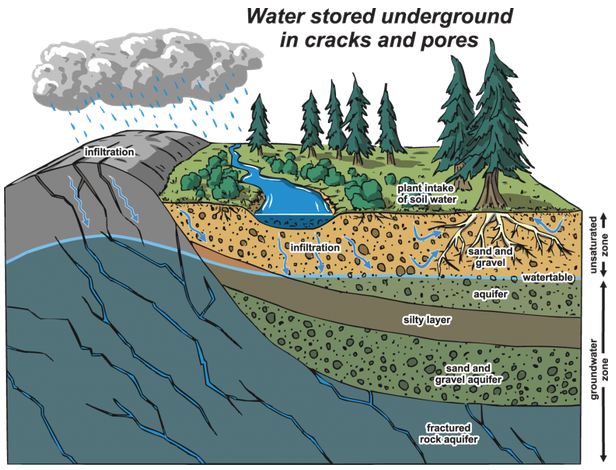
\includegraphics[width=10.8cm, keepaspectratio]{images/aquifers.png}
    \caption{Water cycle}
\end{wrapfigure}
Aquifers lie in the saturated zone below the water table and are the source of 
our drinking water. They are the ``zones in sediments and bedrock that 
receive, store, and transmit significant amounts of water to wells and 
springs``~\citep{haeckel2014}. The area of land that contributes to recharging 
aquifers is called the aquifer recharge area; this area can be as large as an 
entire watershed or a sub-basin. Aquifers also have discharge areas, which feed 
perennial streams, linked ponds/lakes, and riparian wetlands.
\par
With more than 25\% of New Yorkers dependent on groundwater for drinking, 
municipalities have an important role to play in ensuring that drinking water 
remains plentiful and clean. While regional aquifer depletion in New York is 
rare, thanks to our plentiful precipitation, localized depletion can occur when 
withdrawals exceed natural local recharge rates. Municipalities can implement 
protective measures to support a balance between withdrawals and natural 
recharge, thereby protecting wells and the waterbodies that depend on 
groundwater. Municipalities can also foster an awareness of aquifer pollution 
and enact preventive legislation. These efforts can focus on the various sources 
of aquifer pollution: chemical spills; run-off of oil, gas, and antifreeze from 
motor vehicles; road salt; common household cleaners, herbicides, and 
pesticides; underground storage tanks; and improperly spaced or faulty septic 
systems and improperly maintained public sewer systems. An important first step 
can be the development of a management plan for the protection of groundwater; 
the New York Rural Water Association offers technical assistance for the 
development of \href{ 
http://www.nyruralwater.org/sites/default/files/Fact\%20Sheet10\_1-5-2018.pdf}{ 
source water protection plans}.

\subsection*{Public Wells, Aquifers, and Risk Sites Map}
Cornwall is fortunate to be underlain by many below water table aquifers, 
depicted as the pink, green, and brown areas on the map. The Town and Village 
also have four sizable above water table aquifers, appearing as yellow on the 
map. They are located primarily along the Moodna Creek, Woodbury Creek, and on 
the banks of the Hudson River. Orange County Water Authority's 
\href{
http://www.kj-seqra.com/507Acres/ReferenceMaterial/OCWA\%202008\%20Moodna\%20Wat
ershed\%20Atlas\%20(39MB).pdf}{Moodna Creek Watershed Atlas} classified all of 
Cornwall’s aquifers as "Important Groundwater Sources" and, as such, are 
important to drinking water.

\includepdf[pages=-,fitpaper]{cornwall_maps/WellsandRiskSites.pdf}
\label{map:wells}
\namedlabel{map:wellsandrisksites}{Public Wells, Aquifers and Risk Sites Map}
\clearpage
\section*{Wells}\label{subsec:wells}
Cornwall has four sources of drinking water: local surface water from the 
Village of Cornwall-on-Hudson’s reservoirs in Black Rock Forest, surface water 
from New York City’s Catskill Reservoir System via the Catskill Aqueduct, 
private wells, and public wells. This diversity of water sources provides great 
flexibility to provide uninterrupted, high quality drinking water to the Town’s 
residents. It is our most precious natural resource.
\par
Cornwall's public wells are indicated by blue dots on this map, with many lying 
directly over aquifers. They are located along Taylor Road, near the Moodna 
Creek (B3). The map also seems to indicate the presence of two additional wells 
along Angola Road just southwest of Route 9W and near the intersection of Angola 
Road and Mineral Springs Road; however, the Village Water Department has no 
knowledge of wells at that site. The drilling of new wells must be carefully 
monitored for negative effects on surrounding public and private wells. 
Excessive extraction can change stream flow and water temperature, affecting the 
survival and reproduction of aquatic life.

\subsection*{Risk Sites}\label{subsec:risksites}
The map also shows many risk sites. These include petroleum bulk storage 
facilities (brown dots) and remediation sites (pink diagonal lines), many of 
which are located directly over or adjacent to aquifers. There is only one 
chemical bulk storage facility of record located near the aquifer that 
underlays the Cornwall Town Landfill (C2). Removing these bulk storage 
facilities from these sensitive locations should be explored; change in property 
ownership may present opportune times for removal.

The map shows four NYSDEC remediation sites. They include:
\begin{itemize}
    \item The Star Expansion site on Industry Drive in Mountainville, between 
    the NYS Thruway and Woodbury Creek (B4). The Groundwater on-site is 
    contaminated with chlorinate solvents. Public water supply wells are 
    located within 1000 meters of the site, but are hydrogeological 
    upgradient, meaning that any onsite contaminants cannot flow 
    uphill. Private residential wells are located within 200 meters 
    and have shown no contamination. The site presents a significant 
    environmental threat due to the ongoing releases of contaminants from the 
    source areas into the groundwater/soil vapor.
    \item The Majestic Weaving Corporation site, on Mill Street, along the 
    Moodna Creek (C2). Remedial measures taken have removed contamination from 
    the site, therefore exposures to site contaminations are not expected.
    \item The inactive Cornwall Town Landfill site located between the NYS 
    Thruway and Route 32 on Halloran Road on the north side of the Town (C2). 
    The municipal waste landfill was closed in 1977. The site is currently 
    being used for leaf composting and storage of gravel. Nearby wells have 
    been sampled by the Department of Health. No contaminants were found.
    \item The area at the southern tip of the Town, shared by the Towns of 
    Woodbury and Highlands and the location of many unexploded ordinances.
\end{itemize}
% link to GPS coordinates or parcel reference?
The map also shows three \gls{spdes} permitted 
locations (purple diamonds): Star Mountainville Industrial Park (B4) 
discharging into Woodbury Creek and discharges from sewage treatment plants into 
Moodna Creek at C2 and at the mouth of the Moodna (D1). SPDES is a permit 
program that allows permitted businesses, municipalities, and individuals to 
dispose of wastewater under highly regulated conditions to prevent the pollution 
of local waterbodies Proper treatment of wastewater is important to reducing the 
negative impact on water resources.

\chapter{Floodplains}\label{subsec:floodzones}
\subsection*{Why you need this map}
The New York Climate Change Science Clearinghouse notes that the Northeast and 
New York State have seen a 71\% increase in heavy precipitation events that 
have resulted in major and costly flooding. Typically flooding happens in 
low-land areas that are naturally prone to flooding, known as floodplains. These 
areas are next to streams and other waterbodies that can become engorged and 
overflow during heavy rainfalls and snowfalls.
\par
Flood zones are delineated by the \gls{fema} and the US \gls{hud}. Delineated 
flood zones typically include historic floodplains and their floodways. Two 
flood zone categories are commonly used: 100-year and 500-year flood zones. 
Land areas and all structures lying within a 100-year flood zone have a 1\% 
chance of flooding every year; areas within a 500-year floodplain have 0.2\% 
chance of flooding annually. Due to the increased frequency and severity of 
heavy precipitation events, communities throughout the US have seen multiple 
100-year flood events happen in a given year and repeated, annual 500-year 
events. The City of Houston, Texas, for example, has seen three 500-year floods 
in as many years ~\citep{dara2017}.
\par
%% check this
Delineated flood zones, however, are not the only places where flooding can 
happen. Flooding can take place anywhere as a result of poorly designed or 
inadequate culverts and dams (see ~\nameref{subsec:floodzones} section for 
further information). Haeckel and Heady explain that "[d]ue to many variables, 
such as the often-unpredictable nature of floods, local drainage problems, and 
the variable intensity of land development in watersheds, some flood-prone 
areas may not appear on designated floodplain maps, and floodplain designations 
may change over time as more information becomes available." The increase in 
impervious surfaces, like roads, driveways, and buildings, prevent absorption 
of floodwaters and results in increased stormwater run-off into waterways. As 
floodwaters travel over various land uses, pollutants are collected and 
deposited in habitats, thereby degrading them.
\par
Planning around locally known flood-prone areas can help municipalities reduce 
the impact of floods on their communities. Cornwall, for example, has long been 
subject to flooding events that have eroded hillsides, damaged structures, and 
even caused dislocation from businesses and residences. Local governments can 
institute policies and practices that harness the benefits of floodplains, such 
as slowing and storing floodwaters and reducing downstream flood damage, 
through conservative buffering around know flood-prone areas. Other benefits of 
preserved floodplains include creating a natural safety zone for development 
and the damaging impacts of floods. By implementing relevant policies, 
municipalities would also be supporting the plants and animals that "tolerate 
occasional flooding and support the in-stream food web" ~\citep{haeckel2014}.

\subsection*{Flood Zones and Flooded Roads Map}
The most significant floodplain areas in Cornwall are located along the Moodna 
and Woodbury creeks, on the Hudson River shoreline, and along smaller streams 
in residential areas of the Town and Village (see D2). The waterbodies shown on 
the map (springs, lakes, streams) contribute to the Moodna Creek’s flow. The 
Moodna forms in the Town of Blooming Grove, flows through the Village of 
Washingtonville and the Town of Cornwall, ending its path through the Town of 
New Windsor into the Hudson River. It is the culmination of these water sources 
that can also lead to the flooding that has devastated portions of these 
municipalities.
\par
The Flood Zones and Flooded Roads map also shows roads that were closed and/or 
flooded during Hurricane Irene in 2011 (yellow) and the April 2007 spring 
northeaster (red). During these extreme weather events, many properties located 
near the mapped flood zones were flooded – even those that were not in 
delineated flood zones.
\begin{itemize}
    \item Hurricane Irene closed many roads, including all segments of the NYS 
        Thruway that passes through Cornwall, Otterkilll Road, portions of 
        Route 32, Quaker Avenue, Continental Road, Hasbrouck Avenue, 
        the Boulevard, and other smaller local roads.
    \item The April northeaster closed all of Route 9W in Cornwall, along with 
        portions of Otterkill Road and Taylor Road near the Moodna Creek in 
        the western part of the Town.
\end{itemize}
\includepdf[pages=-,fitpaper]{cornwall_maps/FloodZonesandFloodedRoads.pdf}\label{map:floodzonesandfloodedroads}

\chapter{Wetlands}\label{subsec:wetland}
Whether you know them as marshes, swamps, or bogs, the many benefits of 
wetlands to humans, animals, and plants are widely recognized through 
protective governmental legislation, by scientists, and by those who enjoy the 
recreational features supported by wetlands. Some of these benefits include:
\begin{itemize}
    \item Acting as a buffer to control flooding and reduce damage from storm 
    surge.
    \item Serving as naturally-occurring filtration devices, cleansing surface 
    water of impurities.  Wetlands can remove or trap 20-60\% of metals, 80-90\% 
    of sediment, and 70-90\% of nitrogen (Ecological Society of America).
    \item Holding and slowly releasing water from sources like snowmelt, 
    rainfall, or runoff, thereby maintaining base streamflow and recharging 
    groundwater.
    \item Storing 1-1.5 million gallons of floodwater for every acre of wetland
    and supporting 75\% of commercially harvested fish through spawning areas 
    (US Environmental Protection Agency 2001).
    \item Producing food and organic material that supports commercial and 
    sport fisheries. Wetlands also provide "breeding, feeding, and wintering 
    habitat for hundreds of wildlife species," like birds, mammals, and 
    amphibians. (US Army Corps of Engineers 1998)
    \item Recreational activities, like kayaking, canoeing, birdwatching, 
    hunting, and fishing.
    \item Serving as natural "carbon sinks" by helping reduce atmospheric
    greenhouse gases through excess atmospheric carbon storage (Association 
    of State Wetlands Managers).
\end{itemize}

How do wetlands provide these important benefits? Wetlands are defined as "an 
area that is covered by shallow water or has waterlogged soils for long periods 
during the growing season in most years" (USACE 1998). Additionally, wetlands 
must have hydric soils and support "plants that require saturated soils to 
survive\ldots [or that] can tolerate prolonged wet soil conditions" (USACE 
Wetlands Identification). These features enable wetlands to act as, 
essentially, giant sponges. This image shows how wetland soils and their plants 
store water from both surface flow and groundwater flow, slowly releasing it to 
streams or aquifers.
%% image
\begin{wrapfigure}{L}{8.1cm}
    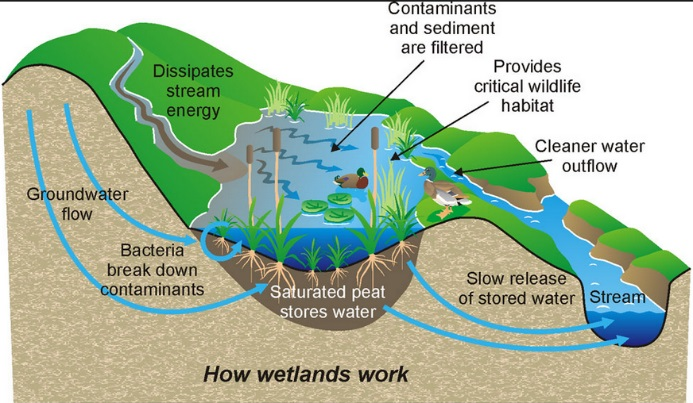
\includegraphics[width=7.9cm, keepaspectratio]{images/wetlands_work.jpg}
  \caption{Wetlands at work}\label{fig:wetlands}
  %\vspace{-10pt}
\end{wrapfigure}
Because of their critical ecological importance, wetlands are regulated by 
Section 404 of the Federal Clean Water Act and NYSDEC's Freshwater Wetlands 
Act. The presence of wetlands is often the reason many development projects are 
subjected to an environmental impact review under federal and/or state laws. The 
Freshwater Wetlands Act protects wetlands, and the 100-foot boundary around 
them, that are larger than 12.4 acres; smaller wetlands of unusual local 
importance are also protected. Many communities in NYS have recognized the 
importance of wetlands by enacting legislation that protects wetlands and vernal 
pools down to 1/10$^{th}$ of an acre through local wetland laws, wetland overlay 
districts, and supplemental zoning standards. The Hudson River Estuary 
Program/Cornell University created a very useful Summary of Municipal Wetland 
and Watercourse Protection Techniques, found in Appendix 
~\nameref{app:cornwall_wetlands}. These wetland protection techniques can address the 
impact that land use decisions can have on wetlands by considering adjacent 
upland areas and connected hydrologic features, like streams.

The sources of wetland data have limitations, requiring public information and 
on-site observations to identify smaller wetlands and confirm regulated wetland 
sized. Haeckel and Heady note that the Federally-designated US Fish and 
Wildlife Service’s National Wetland Inventory "maps often underestimate wetland 
area and omit smaller and drier wetlands." They also note that the NYSDEC's 
Freshwater Wetland Maps were created with "minimal field checking, and are not 
intended to be accurate depictions of the limits of state wetland jurisdiction 
on any site." Both map sources are created by aerial photos analysis.

\subsection*{Wetland Mitigation}
Mitigation, in the broadest sense, is all those actions taken to counter adverse 
effects of a project. The science of restoring, creating, or enhancing wetlands 
in a mitigation context is evolving. We should be cautious about permitting a 
wetland to be altered on the expectation that losses can be fully compensated. 
Protecting wetlands saves money by decreasing flood hazards, reducing the need 
for flood mitigation projects, and decreases the cost of water treatment. 
Priority must be placed on avoiding impacts to existing wetlands and flood 
plains given the uncertainties associated with compensation.

\subsection*{Wetlands and Hydric Soils Map}
This map shows four designations of existing and potential wetlands in the Town 
of Cornwall and the Village of Cornwall-on-Hudson: \gls{nysdec} Wetlands 
(green), NWI Wetlands (purple), Probable Wetlands/Hydric Soils (pink), and 
Possible Wetlands/Somewhat Poorly Drained Soils (light brown). 

Wetlands (green and purple) are primarily located at the bases of the mountains 
of the Hudson Highlands, including Storm King Mountain and Schunnemunk Mountain 
as well as areas within Black Rock Forest. In Cornwall, the largest Wetlands 
areas are located west of Route 32 and near the NYS Thruway (Interstate 87) just 
south of the New Windsor border. Other significant wetlands lie near Orrs Mills 
Road and Route 94, to the west of the Thruway. Of the 722 of NWI-classified 
wetlands in the Town, 57\% are freshwater wetlands and 41\% are estuarine and 
marine deepwater wetlands. For the Village, 98\% are estuarine and marine 
deepwater wetlands. (See Appendix \ref{app:cornwall_wetlands})

Probable Wetlands/Hydric Soils (pink) are found along the shores of the Hudson 
River, the Moodna Creek, Woodbury Creek, Canterbury Brook, and Baby Brook. 
Hydric soils have been mapped because they are areas where there is a 
particularly high potential for additional true wetlands. The widely scattered 
incidence of Possible (light brown) and Probable Wetlands interspersed in 
residential areas of the Town and Village should be carefully evaluated when 
those areas are targeted for any type of development or paving.
\includepdf[pages=-,fitpaper]{cornwall_maps/WetlandsandHydricSoils.pdf}\label{map:wetlandsandhydricsoils}

\chapter{Streams and Water Quality}\label{subsec:streamsquality}
\subsection*{Why you need these maps}
The Town of Cornwall and the Village of Cornwall-on-Hudson have a broad network 
of perennial, intermittent, and ephemeral streams that are admired for their 
beauty. Some are perennial, flowing continuously throughout the seasons, but 
some may dry up during drier periods. These include the Moodna Creek and its 
tributaries flowing from the towns of Blooming Grove and New Windsor; Woodbury 
Creek and its tributaries flowing from the towns of Woodbury and Highlands; and 
Idlewild Creek and its tributaries flowing entirely from within Cornwall. With 
the exception of a few streams, like Clove Creek and the yet-to-be-named creek 
alongside Pagenstecher Park, all streams flow into the Hudson River via the 
Moodna Marsh. All are beautiful, but some are particularly magnificent like Baby 
Brook in Schunnemunk Mountain, pictured at left.
\begin{wrapfigure}[25]{L}{5.7cm} %5.9 5.7
    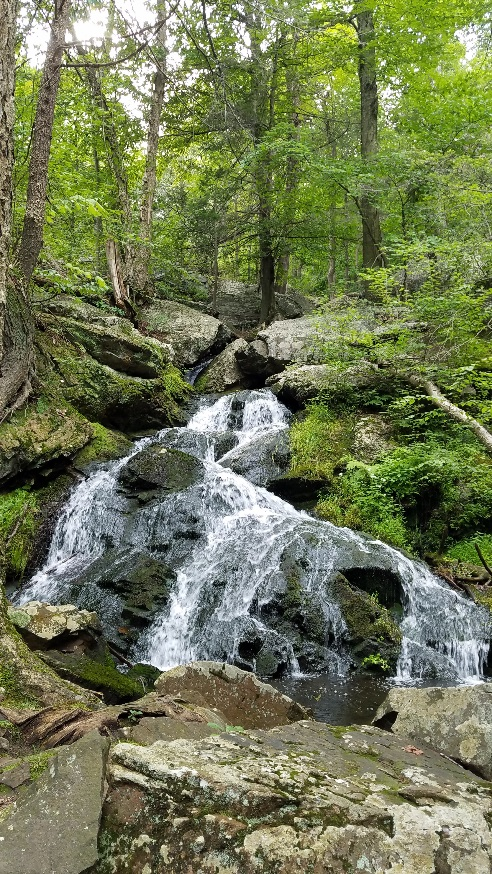
\includegraphics[width=5.5cm, keepaspectratio]{images/stream.jpg}
  \caption{Baby Brook in Schunnemunk Mountain}\label{fig:bablingbrook}
\end{wrapfigure}

Our streams are also important to habitat health, water quality and 
availability for drinking water and irrigation, flood management, and 
recreational enjoyment. Streams add immeasurably to our residents’ quality of 
life and to the value of our properties. Development can result in the 
alteration of streams or modification of their flows from installation of 
culverts and dams. Development can also increase surface water runoff from the 
reduction of permeable surfaces. These changes can increase flooding, increase 
the deposition of pollutants in our waterbodies, and interfere with habitats 
(see ~\nameref{subsec:streamandriparianhabitat} and 
~\nameref{subsec:floodzones} sections). With our changing climate, 
precipitation has become more variable and extreme in the Northeast, 
exacerbating the deposition of a wide range of contaminants into streams and 
other local waterbodies from increased stormwater runoff.
We are informed of the quality of our streams through various measurements and 
classifications established by the federal government through the Clean Water 
Act and New York State through the Environmental Conservation Law. These 
quality assessments are explained through the following two maps: 
(~\nameref{map:streamclassifications}) and Stream Biomonitoring and 
Priority Waterbodies (~\nameref{map:biomonitoringandprioritywaterbodies})

\subsection*{Stream Classification Map}
Freshwater streams and waterbodies are classified by the DEC based on existing 
or best usage from classes AA or A for drinking water (in green on this map) to 
D, which is not suitable for drinking, swimming, nor for supporting fisheries. 
Streams with a classification of A, B, or C may also have a standard of T (may 
support trout) or TS (may support trout spawning). The description of NYSDEC’s 
streams classifications appears below.
\begin{itemize}
    \item AA or A: Used as a source of drinking water (green)
    \item B: Best usage for swimming and other contact recreation, but not for
        drinking (yellow)
    \item C: Waters supporting fisheries and non-contact activities (orange)
    \item D: Lowest classification (not on map)
\end{itemize}
''Waterbodies that are designated as C(T) or higher (e.g., C (TS), B, A, or AA) 
are collectively referred to as protected streams, and are subject to 
additional regulations and require a State permit for disturbance of the bed or 
banks``~\citep{haeckel2014}. As Cornwall has no streams in the D 
classification, all streams are protected. Other systems of stream 
classification are based on a range of physical conditions, habitat values, and 
human uses.

In the Town and Village, well-shaded cool to cold-water streams with clean 
gravel bottoms are able to support native fish such as brook trout. These 
trout-friendly areas are listed below.
\begin{itemize}
    \item Map sections B4/B5, C4/C5: Mineral Spring Brook is currently listed 
as a Class C stream capable of supporting trout spawning (TS).
    \item Map section B4: Woodbury Creek is currently listed as a Class C (TS) 
stream.
    \item Map sections C2/C3: Moodna Creek is currently listed as a Class B (T) 
stream capable of supporting a trout population.
    \item Map sections C2/C3/C4, D2/D3/D4: Idlewild Creek and its tributaries, 
including Black Rock Forest’s Black Rock Brook are classified as Class C (TS) 
and Class B (TS) streams capable of supporting trout spawning.
\end{itemize}

\includepdf[pages=-,fitpaper]{cornwall_maps/StreamClassifications.pdf}\label{map:streamclassifications}

\subsection*{Stream Biomonitoring and Priority 
Waterbodies}\label{subsec:streambiomonitoring}
Surface water has an ecosystem supporting a wide variety of plant and animal 
life. Since this ecosystem is directly affected by the quality and quantity of 
the water in its environment, or stressors on this environment, water quality 
can be determined through biological monitoring or biomonitoring of the variety 
and number of organisms which inhabit waterbodies. These organisms, such as 
fish, invertebrates and plant life, are catalogued by number and type. The 
results determine if the organisms were collected from clean or polluted water 
and are an indicator of the health and safety of a waterbody. Ongoing 
biomonitoring will reveal changes in water quality over time. When surface 
water and wetlands are polluted, or when groundwater is not adequately 
replenished, it ultimately affects our aquifers; biomonitoring can reveal and 
provide the beginning point for addressing such public health issues. In the 
Lower Hudson Basin, agriculture, urban/storm runoff, municipal discharge, and 
hydrologic modification were found to be the primary sources of impact on our 
streams and waterbodies as of 2008 (NYSDEC 2008).

Every major watershed in New York State is studied on a 5-year schedule as part 
of the \gls{ribs} Program. Water quality standards can be upheld through the 
\gls{spdes} permit program, which issues discharge permits and enforces 
compliance in setting DEC Water Quality Classifications.

This map provides information on the Town's and Village's waterbodies via two 
assessment sources: (1) a biomonitoring water quality assessment conducted by 
Orange County Water Authority (2004-2012) applying the Biological Assessment 
Profile score (BAP) and (2) NYSDEC waterbody assessment completed as of 2008.  
NYSDEC and OCWA categorize the biological assessment of water quality in four 
impact categories based on the BAP score. Parameters for developing a BAP score 
include, among others, species richness and diversity, nutrient types and 
levels, and dissolved oxygen levels. BAP assessments reflect an analysis at a 
specific point in time at a specific location. (Additional information on the 
metrics that form the BAP scores is found in NYSDEC's Fact Sheet on Assessment 
of Water Quality Impact on Streams and Rivers.) 

BAP scores appear below. The quality of the streams in Town and Village ranges 
from Moderately Impacted to Non-impacted. There are no Severely Impacted 
streams, although there are several streams that have not been assessed. They 
are generally in protected areas and are Class A streams.
\begin{itemize}
    \item Non-impacted 10-7.5 – Very good water quality. Virtually unaffected 
    by human disturbance or receiving discharges that minimally affect 
    biota.
    \item Slightly Impacted 7.5 – 5 – Good water quality. The 
    macroinvertebrate community is slightly, but not significantly altered from 
    the pristine state.
    \item Moderately Impacted 5-2.5 – Poor water quality. Fish may propagate, 
    but probably will not survive.
    \item Severely Impacted 2.5-0 – Very poor water quality. Only the 
    strongest, most dominant species will survive.
\end{itemize}

The Moodna Creek and its tributaries are mostly Not Impacted (green lines), 
though some in the southwestern part of town have Slight (Minor) Impacts (pink 
lines). Woodbury Creek is also Slightly Impacted.

\includepdf[pages=-,fitpaper]{cornwall_maps/BiomonitoringandPriorityWaterBodies}\label{map:biomonitoringandprioritywaterbodies}
